\documentclass{article}
\usepackage[utf8]{inputenc}
\usepackage{amsmath,amsfonts,amssymb}
\usepackage{listings,import}
\usepackage{algorithm}
\usepackage{algpseudocode}

%Packages
\usepackage[novbox]{pdfsync}
\usepackage{amssymb, amsfonts,mathtools}
\usepackage{eurosym,graphicx,latexsym, amsmath,amsthm,times,nccmath,url}
\usepackage{listings,verbatim,cases}
\usepackage{graphicx,float,fancybox}
\usepackage{epsfig}
\usepackage{epstopdf,tikz}
\usepackage[sans]{dsfont}
\usetikzlibrary{positioning}
\usetikzlibrary{arrows}
\usetikzlibrary{arrows.meta}
\usetikzlibrary{calc}

%\iffalse
%Theorem environments
\newtheorem{theorem}{Theorem}
\newtheorem{lemma}{Lemma}
\newtheorem{proposition}{Proposition}
\newtheorem{corollary}{Corollary}
\newtheorem{remark}{Remark}
\newtheorem{hypothesis}{Hypothesis}
\newtheorem{fact}{Fact}
\newtheorem{example}{Example}
\newtheorem{definition}{Definition}
\newtheorem{open}{Open Problem}
\newtheorem{question}{Question}
\newtheorem{assumption}{Assumption}


%Abreviations of theorem environments
\def\beA{\begin{assumption}}\def\eeA{\end{assumption}}
 \def\beQ{\begin{question}}\def\eeQ{\end{question}}
\def\beD{\begin{definition}} \def\eeD{\end{definition}}
\def\beR{\begin{remark}} \def\eeR{\end{remark}}
\def\beP{\begin{proposition}} \def\eeP{\end{proposition}}
\def\beL{\begin{lemma}} \def\eeL{\end{lemma}}
\def\beC{\begin{corollary}} \def\eeC{\end{corollary}}
  \def\beT{\begin{theorem}}\def\eeT{\end{theorem}}
\def\beXa{\begin{example}} \def\eeXa{\end{example}}
\def\beO{\begin{open}} \def\eeO{\end{open}}

\def\bep{\begin{pmatrix}} \def\eep{\end{pmatrix}}
\def\bev{\begin{vmatrix}} \def\eev{\end{vmatrix}}
\def\BEN{\begin{enumerate}}  \def\BI{\begin{itemize}}
\def\EEN{\end{enumerate}}   \def\EI{\end{itemize}}
\def\bea{\begin{eqnarray*}} \def\eea{\end{eqnarray*}}
\def\bc{\begin{cases}} \def\ec{\end{cases}}
%\def\belst{\begin{lstlisting}[style=mathematica]} \def\eelst{\end{lstlisting}}

\newcommand{\E}{\ensuremath{\mathbb{E}}}
\renewcommand{\P}{\ensuremath{\mathbb{P}}}

\newcommand{\ind}[1]{\ensuremath{\mathbbm{1}_{\left\{#1\right\}}}}
\newcommand{\diff}{\mathop{}\mathopen{}\mathrm{d}}
%\newcommand{\cal}[1]{\ensuremath{\mathcal{#1}}}
\newcommand\croc[1]{\left\langle #1\right\rangle}
\newcommand\steq[1]{\stackrel{\text{\rm #1.}}{=}}

\def\etal{et al.}
\def\eps{\varepsilon}
\def\cadlag{c\`adl\`ag }

%\fi
 %\graphicspath{{images/}}

 \long\def\symbolfootnote[#1]#2{
\begingroup
\def\thefootnote{\fnsymbol{footnote}}\footnote[#1]{#2}
\endgroup}
\def\fn{\symbolfootnote}
\newcommand{\te}[1]{\text{#1}}
 %figure
 \newcommand{\figu}[3]{
\begin{figure}[H]
\centering
\includegraphics[scale=#3]{#1}
\caption{#2\label{f:#1}}
\end{figure}
}

%greek
\def\g{\gamma} \def\G{\Gamma}\def\ga{\gamma} \def\Ga{\Gamma} \def\de{\delta}  \def\b{\beta}\def\va{\bff a }\def\al{\alpha}
\def\a{\alpha}\def\ba{\bff \alpha}
\def\ze{\zeta}  \def\th{\theta} \def\vt{\vartheta}\def\si{\sigma}
\def\si{\sigma} \def\ga{\gamma}
\def\ep{\epsilon}
\def\k{\kappa} \def\la {\lambda}\def\f{\varphi}
\def\La {\Lambda} \def\Lgn{\Lambda+\g_i+\delta}\def\Lg{\Lambda+\g_e}

%Some mathematical commands
\newcommand{\realpos}{\mathbb{R}_{> 0}}
\newcommand{\realnneg}{\mathbb{R}_{\geq 0}}
\newcommand{\naturalpos}{\mathbb{N}_{>0}}
\providecommand{\pr}[1]{\left(#1\right)}
\providecommand{\pp}[1]{\left[#1\right]}
 \newcommand*{\Scale}[2][4]{\scalebox{#1}{$#2$}}
 \newcommand{\be}[1]{\begin{equation}\label{#1}}
\newcommand{\ee}{\end{equation}}

%Enumerations
\newcommand{\beq}{\begin{eqnarray}
    }
\def\eeq{\end{eqnarray}}

%fonts
\newcommand{\mc}[1]{\mathcal{#1}}
\newcommand\blue[1]{\textcolor{blue}{#1}}
\newcommand{\red}{\textcolor[rgb]{1.00,0.00,0.00}}
\newcommand{\green}{\textcolor[rgb]{0.00,1.00,0.00}}

\newcommand{\bff}[1]{{\mbox{\boldmath$#1$}}}
\newcommand\X{\boldsymbol{X}}
\def\x{\boldsymbol{x}}
\newcommand\y{\boldsymbol{y}}
\newcommand\br{\boldsymbol{r}}
\newcommand\by{\boldsymbol{y}}
\newcommand\bd{\boldsymbol{d}}
%\newcommand\bv{\boldsymbol{v}}
\newcommand\bQ{\boldsymbol{Q}}


 \newcommand{\xb}{\x}
\newcommand{\yb}{\y}
\newcommand{\Yb}{{\mathbf{Y}}}
\newcommand{\Ab}{\mathbf{A}}
\newcommand{\zb}{\mathbf{z}}
\newcommand{\Zb}{\mathbf{Z}}
%%% script
\newcommand{\Rs}{{\mathscr R}}
\newcommand{\Ss}{{\mathscr S}}
\newcommand{\Ns}{{\mathscr N}}
\newcommand{\Cs}{\mathscr C}
%%% MATHCAL
\def\mS{{\mathcal S}}\def\mH{{\mathcal H}}\def\mE{{\mathcal E}}
\newcommand{\mC}{\mathcal{C}}\newcommand{\mP}{\mathcal{P}}
\newcommand{\mL}{\mathcal{L}}
\newcommand{\bb}{\mathbf{b}}
\def\mE{\mathcal{E}}\def\mF{\mathcal F}\def\mV{{\mathcal V}} \def\mM{{\mathcal M}}
\def\bi{{ {\bff y}}}  \def\ei{a_i}


\def\bbe{B%{\bff \beta}
} \def\vbe{\vec {\bff \beta}
}
\def\vb{\vec {\bff b}}\newcommand{\e}{\;\mathsf e}
\def\v1{\vec {\bff 1}}
\def\vn{\vec \de} \def\bg{\bff \Gamma}   \def\vz{\vec 0}
\def\rd{\r_{dfe}} \def\sd{\s_{dfe}} \def\dd{D_{dfe}}\def\vd{v_{dfe}} \def\zd{z_{dfe}} \def\xd{\T x_{1}}
\def\ie{i.e. }\def\re{\r^{ee}}\def\se{\s^{ee}}
\def\ye{{\y^{ee}}}\def\xe{{\x^{ee}}}\def\we{\w^{ee}}\def\eE{\e^{ee}}
 \def\for{\forall}\def\I{\infty}\def\prf{{\bf  Proof:}}  \def\QED{\hfill {$\square$}\goodbreak \medskip}
 \def\eqr{\eqref} \def\Eq{\Leftrightarrow} \def\Prf{{\bf  Proof:}}
 \def\no{\nonumber}  \def\fr{\frac} \def\lab{\label}
 \def\De{\Delta} \def\mG{{\mathcal G}}
\def\mR{\mathcal R} \def\mI{\mathcal I}
\newcommand{\R}{\mathbb{R}}
\renewcommand{\r}{ \mathsf r}
\newcommand{\s}{ \mathsf s}
\newcommand{\N}{\mathbb{N}}
\newcommand{\Z}{\mathbb{Z}}
 %\def{\i }{\mathsf i}
\def\vi{\overset{\rightarrow}{\mathsf \i }}
\def\mC{{\mathcal C}}\def\mR{{\mathcal R}} \def\mN{{\mathcal N}} \newcommand{\cH}{{\mathcal H}}\newcommand{\cT}{\mathcal T}\newcommand{\cK}{\mathcal K}
\newcommand{\MN}{\mathbb{N}}
\newcommand{\MR}{\mathbb{R}}\newcommand{\ra}{\rightarrow}
\def\R{\mathcal R}\def\mD{\mathcal D }\newcommand{\MZ}{\mathbb{Z}} \def\vv{\overset{\rightarrow}{v}}
\def\vr{\; \vec {\mathsf r}}\def\bde{\bff \delta}\def\bg{\bff \gamma}
\def\bx{\bff x}
\def\z{\zeta} \def\bz{\bff 0} \def\f{\varphi} \def\T{\widetilde} \def\mT{\mathcal{T}}
\def\eE{\mathsf e_{ee}} \def\de{\delta}\def\eps{\varepsilon}
\def\Roc{R_{1,c}}\def\Rtc{R_{2,c}}
%MathOperators
\DeclareMathOperator{\TV}{TV}
\DeclareMathOperator{\Cov}{Cov}
\DeclareMathOperator{\tr}{tr}
\DeclareMathOperator{\diag}{Diag}
\DeclareMathOperator{\intr}{\mathrm{Int}}

% CRNs defined by S, C, and R
\def\SS{\mathcal S}
\def\CC{\mathcal C}
\def\RR{\mathcal R}
\newcommand\op{\operatorname}
\newcommand{\supp}{\op{supp}}
%\newcommand{\G}{(\SS,\RR)} % the `name' of the CRN
%Some text Abreviations

\def\ece{eco-epidemiological model}\def\para{parameter}
\def\SPF{SIR-PH-FA model}\def\var{variable}
\def\qu{\quad}\def\im{\item} \def\Lra{\Longrightarrow}
 \def\sssec{\subsubsection}  \def\sec{\section} \newcommand{\pdd}[1]{\frac{\partial}{\partial{#1}}}
 \def\ssec{\subsection} \newcommand{\vect}[1]{\boldsymbol{#1}}
\def\elt{element}\def\itc{it is easy to check that }
 \def\brn{basic reproduction number}
\def\com{compartment} \def\AB{$(A,B)$ Arino-Brauer epidemic models}\def\EM{epidemic model}\def\fp{fixed point}
\def\bfp{boundary fixed point}
\def\WRZD{weakly reversible, zero deficiency}
\def\dete{deterministic }\def\corr{corresponding }
 \def\Mp{More precisely, } \def\sats{satisfies} \def\form{formula } \def\saty{satisfy}\def\mbc{may be checked to be}
 \def\wl{without loss of generality}
 \def\fno{from now on} \def\satg{satisfying }
 \def\FHJ{Feinberg-Horn-Jackson} \def\sm{stoichiometric matrix}\def\MTT{matrix tree theorem}
 \def\bzn{basic replacement number}\def\wlo{w.l.o.g.}  \def\ith{it holds that }
\def\Fr{Furthermore, }\def\wms{we must show that }\def\dfe{disease free equilibrium}\def\wmr{we may rewrite }
\def\Nt{Note that }\def\Wmc{We may check that }
\def\mpr{more precisely, } \def\coe{coefficient} \def\fe{for example }
\def\resp{respectively} \def\GMAK{generalized mass action kinetics} \def\DFE{disease free equilibrium}\def\RH{Routh-Hurwitz }
\def\Oth{On the other hand} \def\MM{Michaelis-Menten} \def\ass{assumption}
\def\ACR{absolute concentration robustness} \def\wrt{with respect to }\def\chp{characteristic polynomial}
\def\uph{\red{UP TO HERE}} \def\Itf{It follows that }
\def\eig{eigenvalue}\def\eigv{eigenvector}\def\mbw{may be written as }
\def\mubw{must be written as }\def\sta{stability}
\def\ito{it turns out that }
\def\itf{it follows that}\def\equ{equation}
\newcommand\CRN{chemical reaction network }
\newcommand\RN{reaction network }
\newcommand\BIN{biological interaction network }
\newcommand\CRNNoSpace{chemical reaction network}
\newcommand\CRNs{chemical reaction networks}
\newcommand\CRNsNoSpace{chemical reaction networks}
\newcommand\CRS{chemical reaction system }
\newcommand\CRSs{chemical reaction systems }
\newcommand\CRSsNoSpace{chemical reaction systems} \def\Dt{Descartes type }\def\ME{mathematical epidemiology}
\def\MEE{eco-epidemiology}\def\SPF{SIR-PH-FA model}\def\mgm{multi group model}
\def\NGM{next generation matrix} \def\Ma{{Mathematica}}
\def\enn{essentially nonnegative/positivity preserving}
\def\nny{nonnegativity}\def\ds{differential system}\def\Lm{Laplacian matrix}\def\LyV{Lyapunov Volterra type function} \def\LdS{Lyapunov diagonally stable}\def\EE{endemic point}%\def\cGBC{{\cite{Giulia,BG21}}
\def\dec{decomposition} \def\pa{parameter}
\def\SGT{spectral graph theory} \def\LV{Lotka-Volterra}
\def\GLV{Generalized Lotka-Volterra model}
\def\gLV{generalized Lotka-Volterra model} \def\Lf{Lyapunov function}\def\satd{satisfied}\def\EEP{eco-epidemiological}
\def\nne{non-negative}
\def\PF{Perron-Frobenius} \def\jin{Jacobian matrix of  the invasion vector field with respect to the invasion variables} \def\jrn{Jacobian matrix of  the resident vector field with respect to the resident variables}
\def\jxn{Jacobian matrix of  the $\x$ vector field with respect to the $\x$ variables}
\def\endp{endemic fixed point}
\def\SMW{Sherman–Morrison–Woodbury}\def\qem{quadratic epidemiological model}\def\mbw{may be written as }\def\nz{non zero}
\def\STP{sharp threshold property}\def\gas{global asymptotic stability}
\def\STT{sharp threshold theorem}\def\sksy{skew-symmetric}
\def\How{However, } \def\gene{generalization}
\def\MH{Metzler-Hurwitz } \def\Hur{Hurwitz }\def\H{\hat}\def\cNGM{\cite{AndMay,Diek,Van,Arino,Fall,Bonzi}}
\def\AMG{Anderson May Gupta}\def\CEP{competitive exclusion principle}
\def\GAS{globally asymptotically stable}
\def\LAS{locally asymptotically stable}\def\prop{proportional to }
\def\eiv{eigenvector}\def\edt{expected dwell times}
\def\sus{susceptible}\def\CTMC{continuous time Markov chain}
\def\absC{absorbtion CTMC}\def\LyM{Lyapunov Malkin stable}
\def\coo{coordinate}\def\ABP{$(A,\bbe,P,\f)$ balanced bilinear model}
\def\ABa{$(A,\bbe,\ba,\f)$ balanced bilinear model}
\def\ie{i.e. }\def\pol{polynomial}\def\heu{heuristic}\def\Ito{It turns out that } \def\Itou{It turns out useful to }\def\dec{decomposition}
\def\comp{computation}\def\nim{new infections matrix}\def\wk{well-known}
\def\sys{system}\def\mat{matrix}\def\noni{non-infectious}
\def\rep{representation}\def\prob{probability} \def\DAE{differential algebraic equations} \def\Hb{Hopf bifurcation}\def\enp{endemic point}\def\BTb{Bogdanov-Takens bifurcation}\def\rap{rational approximation}\def\sef{see for example }\def\Kol{Kolmogorov}
\def\frt{furthermore }\def\ch{characteristic polynomial }
\def\Sm{stoichiometric matrix}\def\RLF{robust Lyapunov function}
\def\Mm{Max–Min }\def\nc{non-catalytic}\def\admy{admissibility}
\def\MAR{mass action representation}\def\jac{Jacobi matrix}
\def\reg{regular splitting}\def\nim{new infections matrix}
\def\Itm{It may be checked that }
\def\itm{it may be checked that }\def\sub{substrate}
\def\Me{M_{ee}}\def\dwt{dwell times}\def\pa{\paragraph}
\def\dw{D_w}\def\xy{\x-\y}\def\x{\mathbf{x}}\def\y{\mathbf{y}}
\def\regS{regular splitting}\def\evec{eigenvector} \def\eval{eigenvalue}
\def\fbp{fixed boundary point} \def\fbl{fixed boundary line}
\def\adm{admissible}\def\isd{is defined by}\def\np{\newpage}
\def\spfp{strictly positive fixed  point} \def\RUR{rational univariate representation}\def\oth{otherwise}
\def\how{however}\def\nt{non trivial}\def\fif{forward invariant face}
\def\The{The main hero of mathematical epidemiology (ME) is the DFE}

\usepackage{xcolor,tcolorbox}
\usepackage{geometry}
\geometry{margin=1in}

\lstset{
    language=Mathematica,
    basicstyle=\small\ttfamily,
    keywordstyle=\color{blue},
    commentstyle=\color{gray},
    stringstyle=\color{red},
    breaklines=true,
    frame=single
}

\title{EpidCRN Package  Documentation}
\author{Team}
\date{\today}

\begin{document}

\maketitle
\tableofcontents

\section{Package Overview}

\textbf{EpidCRN} is a Mathematica package for epidemiological models (ME) (whose definition assumes the existence of a unique disease-free boundary fixed point =DFE), which aims to use also Chemical Reaction Network Theory (CRNT) methods.
Models are entered as a pair formed by the  reactions "RN", (which do not depend on the form of the rates), and their rates "rts". The first could be viewed as a definition/standardization of the model, and the second as a secondary feature, which may be chosen as polynomial (mass-action), or  fractional, at the convenience of the author, and depending
on the availability of data.


The main object of study are models with possibly several boundary fixed points 
besides the DFE (or minimal siphons, in CRN terminology), which we call multi-strain.  The focus of our package is somewhat different than that of other similar packages, a major concern being  the flexibility of operating symbolically whenever this is possible (this is a major concern in ME).Once the model is input,   anything should be achievable, at the usual cost. For example,  rational computations of $R_0$ are achieved instantaneously (for multi-strains, this is the max of individual $R_i$ for each strain), but small non-rational $R_0$ may require further effort.  Also, invasion numbers, which appear in stability conditions for the non DFE  boundary fixed points, are instantaneous if rational, but  may require work from the user, if the "siphon"  boundary fixed points are not rational.  Numeric stability scans are also available, in cases where stability is not symbolic, but the user needs to adjust various tolerances, to make this work. In summary, the package aims to provide trivial computations and also less trivial ones, but the latter are at the cost of extra user's time.


\section{Package Structure}

\subsection{Modular Organization}
The package is split into subpackages:

\begin{enumerate}
\item \texttt{EpidCRN.wl} - Main loader package, which contains all the usage statements. The following subpackages are all in the same directory with the loader.
\item \texttt{Core.wl} - Basic network analysis (\texttt{EpidCRN`Core`})
\item \texttt{CRNT.wl} - Chemical reaction network theory (\texttt{EpidCRN`CRNT`})
\item \texttt{Boundary.wl} - NGM and boundary analysis (\texttt{EpidCRN`Boundary`})
\item \texttt{Bifurcation.wl} - Hopf bifurcations and parameter scanning (\texttt{EpidCRN`Bifurcation`})
\item \texttt{Siphons.wl} - Siphon and persistence analysis (\texttt{EpidCRN`Siphons`})
\item \texttt{Utils.wl} - Utility functions (\texttt{EpidCRN`Utils`})
\item \texttt{Visualization.wl} - (\texttt{EpidCRN`Visualization`})
\end{enumerate}

\subsection{Dependency Chain}
\texttt{Core} $\rightarrow$ \texttt{CRNT} $\rightarrow$ \texttt{Boundary} $\rightarrow$ \texttt{Bifurcation} $\rightarrow$ \texttt{Siphons}

\section{Fundamental Functions Reference}

\subsection{Core Functions (EpidCRN`Core`)}

\subsubsection{extMat[reactions]}
Master function extracting network structure.

\textbf{Returns:} \{species, $\alpha$, $\beta$, $\gamma$, $R_v$, RHS, deficiency\}
\begin{enumerate}
\item \textbf{species}: List of species names as strings
\item $\alpha$: Reactant stoichiometric matrix
\item $\beta$: Product stoichiometric matrix
\item $\gamma$: Net stoichiometric matrix ($\beta - \alpha$)
\item $R_v$: Rate vector template
\item \textbf{RHS}: Right-hand side of ODE system
\item \textbf{deficiency}: Network deficiency information
\end{enumerate}

\subsubsection{asoRea[RN]}
Converts reaction network to association format.

\textbf{Input:} \texttt{RN = \{"s"+"i"->2"i", "i"->"r", "r"->"s"\}}\\
\textbf{Returns:} Association with "Substrates"/"Products" keys

\subsubsection{compToAsso[side]}
Parses reaction side to association of species $\rightarrow$ coefficients.

\subsubsection{extSpe[reactions]}
Extracts species list from reaction network.

\subsection{Siphon Analysis (EpidCRN`Siphons`)}

\subsubsection{minSiph[species, asoReactions]}
\textbf{CRITICAL FUNCTION:} Computes minimal siphons (sets of species that become zero at DFE).

\textbf{Input:}
\begin{enumerate}
\item \texttt{species}: List of species names as strings
\item \texttt{asoReactions}: Output of \texttt{asoRea[RN]}
\end{enumerate}

\textbf{Returns:} List of lists of species names as strings\\
\textbf{Example:} \texttt{\{\{"x2"\}, \{"B1","S1"\}, \{"B2","S2"\}\}}

\begin{verbatim}
{spe, al, be, gam, Rv, RHS, def} = extMat[RN];
mS = minSiph[spe, asoRea[RN]];
(* mS contains variable names, NOT indices *)
\end{verbatim}

\textbf{Critical Note:} \texttt{minSiph} returns variable names as strings. Do NOT convert to indices in downstream functions.

\subsection{CRNT Functions (EpidCRN`CRNT`)}

\subsubsection{getComE[RN\_List]}
Extract complexes and edges from reaction network.

\begin{lstlisting}
getComE[RN_List] := Module[{complexes, edges},
  complexes = {};
  edges = {};
  Do[
    Module[{left, right},
      left = RN[[i, 1]];
      right = RN[[i, 2]];
      If[! MemberQ[complexes, left], AppendTo[complexes, left]];
      If[! MemberQ[complexes, right], AppendTo[complexes, right]];
      AppendTo[edges, {left, right}];
    ],
    {i, Length[RN]}
  ];
  {complexes, edges}
];
\end{lstlisting}

\textbf{Input:} Reaction network as list of \{left, right\} pairs\\
\textbf{Returns:} \texttt{\{complexes, edges\}}\\
\textbf{Example:} \texttt{getComE[\{\{a,b\},\{b,c\},\{c,a\}\}]} $\rightarrow$ \texttt{\{\{a, b, c\}, \{\{a, b\}, \{b, c\}, \{c, a\}\}\}}

\subsubsection{IaFHJ[vert\_, edg\_]}
Incidence matrix analysis for FHJ graphs.

\begin{lstlisting}
IaFHJ[vert_, edg_] := Module[{gg, oU, taF},
  gg[a_, b_] := Which[
    a === b[[1]], -1,
    a === b[[2]], 1,
    True, 0
  ];
  oU = Table[
    gg[vert[[i]], edg[[j]]],
    {i, Length[vert]},
    {j, Length[edg]}
  ];
  taF = TableForm[
    oU,
    TableHeadings -> {vert, edg},
    TableAlignments -> {Right, Top}
  ];
  {oU, taF}
];
\end{lstlisting}

\textbf{Input:} Vertices and edges lists\\
\textbf{Returns:} \texttt{\{matrix (n\_complexes $\times$ n\_reactions), tableForm\}}

\subsubsection{IkFHJ[vert\_, edg\_, tk\_]}
Ik matrix computation for FHJ analysis.

\begin{lstlisting}
IkFHJ[vert_, edg_, tk_] := Module[{tri, gg, oU},
  tri = MapThread[Append, {edg, tk}];
  gg[a_, b_] := Which[
    a === b[[1]], b[[3]],
    a === b[[2]], 0,
    True, 0
  ];
  oU = Table[
    gg[vert[[i]], tri[[j]]],
    {i, Length[vert]},
    {j, Length[tri]}
  ] // Transpose
];
\end{lstlisting}

\textbf{Input:} Vertices, edges, and rate constants\\
\textbf{Returns:} Matrix (n\_reactions $\times$ n\_complexes)

\subsubsection{SpeComInc[spec\_, comp\_]}
Species-complex incidence matrix.

\begin{lstlisting}
SpeComInc[spec_, comp_] := Coefficient[#, spec] & /@ comp;
\end{lstlisting}

\textbf{Input:} Species list and complexes list\\
\textbf{Returns:} Coefficient matrix\\
\textbf{Example:} \texttt{SpeComInc[\{x, y\}, \{x + y, 2 x, y\}]} $\rightarrow$ \texttt{\{\{1, 1\}, \{2, 0\}, \{0, 1\}\}}

\subsubsection{lapK[RN\_, rates\_]}
Main Laplacian computation function.

\begin{lstlisting}
lapK[RN_, rates_] := Module[{complexes, edges, laplacian},
  {complexes, edges} = getComE[RN];
  laplacian = IkFHJ[complexes, edges, rates];
  laplacian
];
\end{lstlisting}

\textbf{Input:} Reaction network and rate constants\\
\textbf{Returns:} Laplacian matrix (n\_complexes $\times$ n\_complexes)

\section{Boundary Analysis Functions}

\subsection{NGM[mod, inf]}
Next Generation Matrix analysis.

\textbf{Input:}
\begin{enumerate}
\item \texttt{mod}: \texttt{\{RHS, var, par\}}
\item \texttt{inf}: List of infected compartment indices
\end{enumerate}

\textbf{Returns:} \texttt{\{Jx, Jy, ..., K, ...\}} where \texttt{K = ngm[[4]]} is the transmission matrix

\subsection{Current Session Work: Enhanced Boundary Analysis Modules}

\subsubsection{bdAn[RN, rts] - Simplified Analysis Module}
Core analysis without boundary fixed point computation.

\begin{lstlisting}
bdAn[RN_, rts_] := Module[{
    spe, al, be, gam, Rv, RHS, def, var, par, cp, cv, ct,
    mSi, mSiIndices, inf, mod, K, eig, R0A, cDFE, RDFE, eq0, var0, E0,
    Jx, Jy, eigenSystem, eigenvals, eigenvecs, nonzeroIndices,
    relevantEigenvals, strainAssociation, sortedPairs, mSiNGM,
    ngm
   },

   {spe, al, be, gam, Rv, RHS, def} = extMat[RN];
   var = ToExpression[spe];
   RHS = gam . rts;
   par = Par[RHS, var];
   cp = Thread[par > 0];
   cv = Thread[var >= 0];
   ct = Join[cp, cv];

   (* Direct assignment - mSi contains variable names as strings *)
   mSi = minSiph[spe, asoRea[RN]];
   mSiIndices = Map[Flatten[Position[spe, #] & /@ #] &, mSi]; (* Indices for NGM *)
   inf = Union[Flatten[mSiIndices]];

   (* Compute DFE *)
   cDFE = Flatten[Thread[ToExpression[#] -> 0] & /@ mSi];
   RDFE = RHS /. cDFE;
   eq0 = Thread[RDFE == 0];
   var0 = Complement[var, var[[inf]]];
   E0 = Join[Solve[eq0, var0] // Flatten, Thread[var[[inf]] -> 0]];

   (* Compute NGM *)
   mod = {RHS, var, par};
   ngm = NGM[mod, inf];
   Jx = ngm[[1]] // FullSimplify;
   Jy = ngm[[5]] // FullSimplify;
   K = ngm[[4]] // FullSimplify;

   (* Get eigenvalues and organize by strain *)
   eigenSystem = Eigensystem[K];
   eigenvals = eigenSystem[[1]];
   eigenvecs = eigenSystem[[2]];
   nonzeroIndices = {};
   Do[If[eigenvals[[i]] =!= 0, AppendTo[nonzeroIndices, i]],
      {i, Length[eigenvals]}];

   If[Length[nonzeroIndices] > 0,
    relevantEigenvals = eigenvals[[nonzeroIndices]];
    mSiNGM = Table[Flatten[Table[Position[inf, mSiIndices[[i]][[j]]][[1,1]],
      {j, Length[mSiIndices[[i]]]}]], {i, Length[mSiIndices]}];
    strainAssociation = Table[Module[{strain1Nonzeros, strain2Nonzeros, evec},
       evec = eigenvecs[[nonzeroIndices[[i]]]];
       strain1Nonzeros = Count[evec[[mSiNGM[[1]]]], Except[0]];
       strain2Nonzeros = Count[evec[[mSiNGM[[2]]]], Except[0]];
       If[strain1Nonzeros > strain2Nonzeros, 1,
        If[strain2Nonzeros > strain1Nonzeros, 2, i]]],
       {i, Length[relevantEigenvals]}];
    sortedPairs = Sort[Transpose[{strainAssociation, relevantEigenvals}]];
    R0A = sortedPairs[[All, 2]];,
    R0A = {};];

   {RHS, var, par, cp, mSi, Jx, Jy, E0, K, R0A}
]
\end{lstlisting}

\textbf{Returns:} \texttt{\{RHS, var, par, cp, mSi, Jx, Jy, E0, K, R0A\}}

\section{bdFp Module Usage Guide}

\subsection{Purpose}
\texttt{bdFp} computes boundary fixed points on siphon facets for epidemic models, separating rational solutions from algebraic ones and providing scalar elimination equations for non-rational cases.

\subsection{Syntax}
\begin{lstlisting}
bdfpT = bdFp[RHS, var, mSi]
\end{lstlisting}

\subsection{Parameters}

\subsubsection{Required Inputs}
\begin{enumerate}
\item \textbf{RHS}: Right-hand side vector of the ODE system (from \texttt{bdAn})
\item \textbf{var}: List of all variables as symbols (from \texttt{bdAn})
\item \textbf{mSi}: Minimal siphons as variable names (strings) (from \texttt{bdAn})
\end{enumerate}

\subsection{Output Format}
Returns a list of pairs, one for each siphon facet:
\begin{lstlisting}
{
  {rationalSols1, scalarEq1},
  {rationalSols2, scalarEq2},
  ...
}
\end{lstlisting}

\subsubsection{Output Components}
\begin{enumerate}
\item \textbf{rationalSols}: List of rational solutions (rules like \texttt{\{x -> value, y -> value\}})
\item \textbf{scalarEq}:
\begin{enumerate}
\item \texttt{None} if all solutions are rational
\item Factored polynomial equation if non-rational solutions exist
\item \texttt{"froze"} if computation timed out
\end{enumerate}
\end{enumerate}

\subsection{Example Usage}

\subsubsection{Basic Usage}
\begin{lstlisting}
(* Get core analysis, pass var and gam to preserve order *)
{RN, rts, spe, alp, bet, gam} = ODE2RN[RHS1, var];
{RHS, var, par, cp, mSi, Jx, Jy, cDFE, E0, K, R0A, infVars, ngm} = bdAn[RN, rts, var, gam];

(* Compute boundary fixed points *)
bdfpT = bdFp[RHS, var, mSi];

(* Extract results for each facet *)
facet1Results = bdfpT[[1]];  (* {rationalSols, scalarEq} for first siphon *)
facet2Results = bdfpT[[2]];  (* {rationalSols, scalarEq} for second siphon *)
\end{lstlisting}

\subsubsection{Accessing Results}
\begin{lstlisting}
(* Get rational solutions for facet 1 *)
rationalSols1 = bdfpT[[1]][[1]];

(* Get scalar equation for facet 1 (if any) *)
scalarEq1 = bdfpT[[1]][[2]];

(* Check if facet has only rational solutions *)
If[bdfpT[[2]][[2]] === None,
  Print["Facet 2 has only rational solutions"],
  Print["Facet 2 has algebraic solutions satisfying: ", bdfpT[[2]][[2]]]
];
\end{lstlisting}

\subsection{Example Output}

\subsubsection{Console Output}
\begin{verbatim}
bdFp finds the fixed points on siphon facets are
fps on siphon facet {i1} are {{i_2->0, s->\Lambda/(\mu+\rho), v_1->(\Lambda\rho)/(\mu(\mu+\rho))}},
and 2 more fps satisfying the scalar equation i_2^2(\beta_v\gamma_2 + \mu)(\beta_2 i_2 - \Lambda + \mu) == 0
fps on siphon facet {i2} are {{rational solution 1}, {rational solution 2}}
\end{verbatim}

\subsubsection{Return Value}
\begin{lstlisting}
{
  {
    {{i_2->0, s->\Lambda/(\mu+\rho), v_1->(\Lambda\rho)/(\mu(\mu+\rho))}},
    i_2^2(\beta_v\gamma_2 + \mu)(\beta_2 i_2 - \Lambda + \mu) == 0
  },
  {
    {{solution1}, {solution2}},
    None
  }
}
\end{lstlisting}

\subsection{Interpretation Guide}

\subsubsection{Rational Solutions}
\begin{enumerate}
\item Direct algebraic expressions in terms of parameters
\item Can be used immediately for analysis
\item Represent equilibria with explicit formulas
\end{enumerate}

\subsubsection{Scalar Equations}
\begin{enumerate}
\item Factored polynomial constraints for non-rational solutions
\item Polynomial degree indicates number of solutions
\item Factors reveal mathematical structure
\item Solutions involve radicals, roots, or complex expressions
\end{enumerate}

\subsubsection{Special Cases}
\begin{enumerate}
\item \textbf{"froze"}: Computation exceeded 10-second timeout
\item \textbf{None}: All solutions are rational (no scalar equation needed)
\item \textbf{Empty rational list \{\}}: All solutions are non-rational
\end{enumerate}

\subsection{Common Workflow}

\begin{lstlisting}
(* 1. Load model and get core analysis *)
{RHS, var, par, cp, mSi, Jx, Jy, cDFE, E0, K, R0A, infVars, ngm} = bdAn[RN, rts];

(* 2. Compute boundary fixed points *)
bdfpT = bdFp[RHS, var, mSi];

(* 3. Extract and analyze results *)
Do[
  {rationalSols, scalarEq} = bdfpT[[i]];
  Print["Siphon ", i, ":"];
  Print["  Rational solutions: ", Length[rationalSols]];
  If[scalarEq =!= None,
    Print["  Non-rational solutions satisfy: ", scalarEq];
  ];
, {i, Length[bdfpT]}];

(* 4. Use rational solutions for further analysis *)
rationalEquilibria = Flatten[bdfpT[[All, 1]], 1];
\end{lstlisting}

\subsection{Error Handling}

\subsubsection{Timeout Protection}
\begin{enumerate}
\item 10-second timeout for main \texttt{Solve} operation
\item 3-second timeout for elimination step
\item Returns \texttt{"froze"} for timed-out computations
\end{enumerate}

\subsubsection{Common Issues}
\begin{enumerate}
\item \textbf{Empty results}: Check that \texttt{mSi} contains valid siphon names
\item \textbf{All "froze"}: System may be too complex; try simpler parameter values
\item \textbf{No scalar equation}: Normal if all solutions are rational
\end{enumerate}

\subsection{Integration with bdAn/bd2}

\subsubsection{With bdAn (Core Analysis)}
\begin{lstlisting}
coreResults = bdAn[RN, rts];
{RHS, var, par, cp, mSi, Jx, Jy, cDFE, E0, K, R0A, infVars, ngm} = coreResults;
bdfpT = bdFp[RHS, var, mSi];
\end{lstlisting}

\subsubsection{With bd2 (Complete Analysis)}
\begin{lstlisting}
fullResults = bd2[RN, rts];
{RHS, var, par, cp, mSi, Jx, Jy, E0, ngm, R0A, EA, bdfpT} = fullResults;
(* bdfpT already computed by bd2 *)
\end{lstlisting}

\subsection{Performance Notes}
\begin{enumerate}
\item Runtime scales with system complexity and siphon count
\item Elimination step may be slow for high-dimensional systems
\item Factorization improves readability but adds computational cost
\item Consider using \texttt{bdAn} alone for preliminary analysis if speed is critical
\end{enumerate}



\subsubsection{bd2[RN, rts] - Complete Analysis Module}
Complete analysis combining bdAn + bdFp.

\begin{lstlisting}
bd2[RN_, rts_] := Module[{
    coreResults, RHS, var, par, cp, mSi, Jx, Jy, E0, ngm, R0A,
    bdfpT, EA
   },

   (* Get core analysis from bdAn *)
   coreResults = bdAn[RN, rts];
   {RHS, var, par, cp, mSi, Jx, Jy, E0, ngm, R0A} = coreResults;

   (* Compute boundary fixed points using bdFp with timeout protection *)
   bdfpT = bdFp[RHS, var, mSi];

   (* Create EA structure for backward compatibility *)
   EA = Table[
     Module[{siphonVars, remainingVars},
       siphonVars = ToExpression[mSi[[j]]];
       remainingVars = Complement[var, siphonVars];
       {Thread[RHS /. Thread[siphonVars -> 0] == 0], remainingVars}
     ], {j, Length[mSi]}];

   (* Return complete results *)
   {RHS, var, par, cp, mSi, Jx, Jy, E0, ngm, R0A, EA, bdfpT}
]
\end{lstlisting}

\textbf{Returns:} \texttt{\{RHS, var, par, cp, mSi, Jx, Jy, E0, ngm, R0A, EA, bdfpT\}}

\section{Invasion Graph Theory Implementation}

\subsection{Theoretical Foundation}

Invasion graphs provide a framework for understanding global dynamics of multi-strain epidemic systems by mapping which strains can invade established equilibria. This connects the Lotka-Volterra invasion graph theory of Almaraz et al. with epidemiological invasion numbers.

\subsection{Key Definitions}

\subsubsection{Admissible Communities}
For epidemic models, an admissible community corresponds to a biologically meaningful endemic state where certain strains are present.

\subsubsection{Invasion Rates}
For community $I$ with equilibrium $\mathbf{u}^*$, the invasion rate of strain $j \notin I$ is:
$$r_j(I) = b_j + \sum_{k \in I} a_{jk} u_k^*$$

\subsubsection{Invasion Numbers (Epidemic Context)}
For Rahman-type models:
$$R_j^{(i)} = \mathcal{R}_j \times s_i$$
where $\mathcal{R}_j = \beta_j/\nu_j$ and $s_i$ is susceptible level at equilibrium $i$.

\subsection{Equivalence Theorem}

\textbf{Key Result:} LV invasion rates and epidemic invasion numbers are equivalent:
$$r_j^{\text{LV}}(I) = \nu_j(R_j^{(i)} - 1)$$

\textbf{Sign Correspondence:}
\begin{align}
r_j^{\text{LV}}(I) > 0 &\Leftrightarrow R_j^{(i)} > 1 \quad \text{(successful invasion)}\\
r_j^{\text{LV}}(I) < 0 &\Leftrightarrow R_j^{(i)} < 1 \quad \text{(failed invasion)}
\end{align}

\subsection{Implementation Algorithm}

\begin{lstlisting}
invasionGraph[RHs_, var_, par_, mSi_] := Module[{
    communities, invasionRates, edges
   },

   (* 1. Identify all admissible communities *)
   communities = findAdmissibleCommunities[RHS, var, mSi];

   (* 2. For each community, compute invasion rates *)
   invasionRates = Table[
     computeInvasionRates[RHS, var, communities[[i]]],
     {i, Length[communities]}];

   (* 3. Construct edges based on invasion success *)
   edges = {};
   Do[
     invasiveSets = Position[invasionRates[[i]], _?Positive];
     Do[AppendTo[edges, communities[[i]] -> communities[[j]]],
        {j, invasiveSets}];,
     {i, Length[communities]}];

   {communities, invasionRates, edges}
]
\end{lstlisting}

\subsection{Rahman Model Implementation}

\begin{lstlisting}
rahmanInvasionGraph[E1t_, E2t_, R0A_, E0_] := Module[{
    R01, R02, R12, R21, S1, S2, invasionMatrix
   },

   (* Extract basic reproduction numbers *)
   {R01, R02} = R0A /. E0;

   (* Extract susceptible levels at single-strain equilibria *)
   S1 = (* Extract S level from E1t *);
   S2 = (* Extract S level from E2t *);

   (* Compute invasion numbers *)
   R12 = R0A[[1]] /. E2t; (* Strain 1 invading strain 2 *)
   R21 = R0A[[2]] /. E1t; (* Strain 2 invading strain 1 *)

   (* Construct invasion graph based on thresholds *)
   invasionMatrix = {
     {"DFE", If[R01 > 1, "E1", ""], If[R02 > 1, "E2", ""]},
     {"E1", "", If[R12 > 1, "Coexistence", ""]},
     {"E2", If[R21 > 1, "Coexistence", ""], ""}
   };

   {R01, R02, R12, R21, invasionMatrix}
]
\end{lstlisting}

\section{Bifurcation Analysis Functions}

\subsection{fpHopf[RHS, var, par, p0val]}
Fixed point finder with Hopf analysis.

\textbf{Returns:} \texttt{\{posSols, complexEigs, angle, eigs\}}
\begin{enumerate}
\item \textbf{angle}: \texttt{ArcTan[Re/Im]*180/Pi} (negative = stable focus, positive = Hopf)
\end{enumerate}

\subsection{Parameter Space Scanning Functions}

\subsubsection{scan Function}
The \texttt{scan} function represents the most sophisticated parameter scanning approach:

\begin{verbatim}
{finalPlot, noSolPoints, results} = scan[RHS, var, par, persRule, plotInd,
  mSi, gridRes, steadyTol, stabTol, chopTol, R01, R02, R12, R21]
\end{verbatim}

\textbf{Key Features:}
\begin{enumerate}
\item Automatic variable detection from minimal siphons (\texttt{mSi})
\item Dual scanning modes: Grid mode (fixed resolution) and range mode (adaptive stepping)
\item Comprehensive equilibrium classification: DFE, E1, E2, EE-Stable, EE-Unstable, NoSol
\item Reproduction number integration with R-curve overlays
\item Robust numerical methods with timeouts and error handling
\end{enumerate}

\subsubsection{scanPar Function}
Simpler, more direct scanning approach:

\begin{verbatim}
{finalPlot, errors, results} = scanPar[RHS, var, par, p0val, plotInd,
  gridRes, plot, hTol, delta, wRan, hRan, R01, R02, R21, R12]
\end{verbatim}

\section{Critical Usage Notes}

  \begin{tcolorbox}[colback=red!5!white,colframe=red!75!black,title=Critical Variable Handling Rules]
\begin{enumerate}
    \item \textbf{mSi contains variable names as strings}, not indices
    \item Species names should be strings ("s", "i1", "i2")
    \item Use \texttt{ToExpression[mSi[[j]]]} to convert to symbols when needed
    \item NEVER convert \texttt{mSi} to indices in \texttt{bdAn} or related functions
\end{enumerate}
\end{tcolorbox}

\subsection{Matrix Conventions}
\begin{enumerate}
\item $\alpha$: reactant stoichiometric matrix (species $\times$ reactions)
\item $\beta$: product stoichiometric matrix
\item $\gamma = \beta - \alpha$: net stoichiometric matrix
\item Laplacian follows CRNT convention (column sums = 0)
\end{enumerate}

\subsection{Function Compatibility}
\begin{enumerate}
\item Functions expect exact expression matching using \texttt{===} operator
\item Most functions return lists, not associations
\item Always use timeout protection for \texttt{Solve} operations in boundary analysis
\item Check for rational solutions using \texttt{FreeQ[sol, Sqrt | Power[\_, Except[\_Integer]] | Root | \_Complex]}
\end{enumerate}

\section{Complete Analysis Workflow}

\begin{lstlisting}
(* 1. Load package *)
<< EpidCRN`;

(* 2. Define model *)
RN = {0 -> "s", "s" + "i1" -> 2*"i1", "s" + "i2" -> 2*"i2",
      "s" -> 0, "i1" -> 0, "i2" -> 0};
rts = {La, be1*s*i1/(1+a1*i1), be2*s*i2/(1+a2*i2),
       mu*s, (mu+ga1)*i1, (mu+ga2)*i2};

(* 3. Core analysis (fast, no boundary points) *)
{RHS, var, par, cp, mSi, Jx, Jy, cDFE, E0, K, R0A, infVars, ngm} = bdAn[RN, rts];

(* 4. Complete analysis (with boundary points and timeout protection) *)
{RHS, var, par, cp, mSi, Jx, Jy, E0, ngm, R0A, EA, bdfpT} = bd2[RN, rts];

(* 5. Extract reproduction numbers *)
{R01, R02} = R0A /. E0;

(* 6. Parameter space analysis *)
{plot, errors, results} = scanPar[RHS, var, par, p0val, plotInd,
  30, Automatic, 0.01, 1/20, 0.5, 0.5, R01, R02, R21, R12];

(* 7. Bifurcation analysis *)
{bestAngle, bestValues, finalP0Val} =
  optHopf[RHS, var, par, coP, {3,4}, 120, "NelderMead", 4, 4, 500];

(* 8. Invasion graph construction *)
{communities, invasionRates, edges} = invasionGraph[RHS, var, par, mSi];
\end{lstlisting}

\section{File Structure}

\begin{verbatim}
EpidCRN/
    EpidCRN.wl       (main package loader)
    Core.wl          (EpidCRN`Core` context)
    CRNT.wl          (EpidCRN`CRNT` context)
    Boundary.wl      (EpidCRN`Boundary` context)
    Bifurcation.wl   (EpidCRN`Bifurcation` context)
    Siphons.wl       (EpidCRN`Siphons` context)
    Utils.wl         (EpidCRN`Utils` context)
    Visualization.wl (EpidCRN`Visualization` context)
\end{verbatim}

\textbf{Critical:} File names must match subcontext names exactly for \texttt{Get[]} to work automatically.

\section{Notes for Future Development}

\begin{enumerate}
\item This documentation preserves all fundamental functions with complete code to prevent package modification errors
\item The \texttt{mSi = mS} assignment in \texttt{bdAn} is critical - do NOT convert to indices
\item All timeout protections and rational solution filtering have been thoroughly tested
\item The invasion graph framework provides a unified approach to understanding multi-strain dynamics
\item Function compatibility and variable handling rules must be strictly followed
\end{enumerate}

\section{Antigenic Variation Models}

\subsection{Trypanosoma Model (TrypN.nb)}

\subsubsection{typAnt[RN, rts] - Trypanosoma Antigenic Variation Analysis}

\textbf{Purpose:} Analyzes two-strain Trypanosoma brucei models with antigenic variation through Variant Surface Glycoprotein (VSG) switching.

\textbf{Model Structure:}
\begin{itemize}
\item \textbf{s}: Susceptible host population
\item \textbf{i1, i2}: Infected with VSG variant 1 or 2
\item \textbf{r1, r2}: Recovered from variant 1 or 2
\item Includes recruitment, infection, recovery, death, and waning immunity
\end{itemize}

\textbf{Usage:}
\begin{lstlisting}
<< EpidCRN`;
(* Define reaction network and rates as in TrypN.nb *)
{RHS, var, par, cp, mSi, Jx, Jy, E0, K, R0A} = typAnt[RN, rts];
\end{lstlisting}

\textbf{Returns:}
\begin{enumerate}
\item \textbf{RHS}: Right-hand side of ODE system
\item \textbf{var}: Variable list \{s, i1, i2, r1, r2\}
\item \textbf{par}: Parameter list
\item \textbf{cp}: Parameter constraints (all positive)
\item \textbf{mSi}: Minimal siphons (infection compartments)
\item \textbf{Jx, Jy}: Jacobian blocks
\item \textbf{E0}: Disease-free equilibrium
\item \textbf{K}: Next generation matrix
\item \textbf{R0A}: Basic reproduction numbers for each variant
\end{enumerate}

\textbf{Key Features:}
\begin{itemize}
\item Strain-specific reproduction numbers $R_{01}, R_{02}$
\item Automatic detection of minimal siphons
\item NGM analysis for multi-strain dynamics
\item Foundation for invasion graph analysis
\end{itemize}

\subsection{Recker Model (ReckerN.nb)}

\subsubsection{recAnt[RN, rts] - Recker Antigenic Variation Analysis}

\textbf{Purpose:} Analyzes multi-strain pathogen models with antigenic variation following Recker et al. framework for malaria and other pathogens with antigenic diversity.

\textbf{Model Structure:}
\begin{itemize}
\item \textbf{s}: Susceptible population
\item \textbf{i1, i2, i3}: Infected with antigenic variant 1, 2, or 3
\item \textbf{r1, r2, r3}: Recovered with variant-specific immunity
\item Cross-immunity between variants (implicit in structure)
\item Waning immunity allowing reinfection
\end{itemize}

\textbf{Usage:}
\begin{lstlisting}
<< EpidCRN`;
(* Define 3-strain reaction network and rates as in ReckerN.nb *)
{RHS, var, par, cp, mSi, Jx, Jy, E0, ngm, R0A, EA, bdfpT} = recAnt[RN, rts];
\end{lstlisting}

\textbf{Returns:} Same as \texttt{bd2} output (complete boundary analysis):
\begin{enumerate}
\item \textbf{RHS}: ODE system right-hand side
\item \textbf{var}: Variables \{s, i1, i2, i3, r1, r2, r3\}
\item \textbf{par}: Parameters
\item \textbf{cp}: Parameter constraints
\item \textbf{mSi}: Minimal siphons (infection states)
\item \textbf{Jx, Jy}: Jacobian blocks
\item \textbf{E0}: Disease-free equilibrium
\item \textbf{ngm}: Full NGM structure
\item \textbf{R0A}: Basic reproduction numbers for variants
\item \textbf{EA}: Endemic equilibria structure
\item \textbf{bdfpT}: Boundary fixed points with rational solutions and scalar equations
\end{enumerate}

\textbf{Key Features:}
\begin{itemize}
\item Three antigenic variants with full CRNT analysis
\item Boundary fixed points on siphon facets
\item Rational and algebraic solution separation
\item Supports invasion number computation for multi-strain coexistence
\item Compatible with parameter scanning and bifurcation analysis
\end{itemize}

\subsection{Comparison: typAnt vs recAnt}

\begin{tabular}{|l|l|l|}
\hline
\textbf{Feature} & \textbf{typAnt} & \textbf{recAnt} \\
\hline
Application & Trypanosoma (VSG) & General antigenic variation \\
Number of strains & 2 & 3 (extensible) \\
Function call & Direct implementation & Wrapper for bd2 \\
Boundary points & No (uses bdAn logic) & Yes (full bd2 output) \\
Computation time & Faster & Slower (includes bdFp) \\
Use case & Quick R0 analysis & Complete equilibrium analysis \\
\hline
\end{tabular}

\subsection{Antigenic Variation Analysis Workflow}

\begin{lstlisting}
(* 1. Load package *)
<< EpidCRN`;

(* 2. Define model - use TrypN.nb or ReckerN.nb as template *)
RN = {...};  (* reaction network *)
rts = {...}; (* rate expressions *)

(* 3. For quick analysis: use typAnt *)
{RHS, var, par, cp, mSi, Jx, Jy, E0, K, R0A} = typAnt[RN, rts];
Print["R0 values: ", R0A /. E0];

(* 4. For complete analysis: use recAnt *)
{RHS, var, par, cp, mSi, Jx, Jy, E0, ngm, R0A, EA, bdfpT} = recAnt[RN, rts];
Print["Boundary equilibria: ", bdfpT];

(* 5. Invasion numbers for coexistence analysis *)
(* Extract boundary equilibria and compute invasion conditions *)
\end{lstlisting}

\subsection{Implementation Notes}

\begin{enumerate}
\item Both functions follow EpidCRN naming convention: short abbreviations returning lists
\item \texttt{typAnt} = "Trypanosoma Antigenic variation"
\item \texttt{recAnt} = "Recker Antigenic variation"
\item All outputs are lists (not associations) for consistency
\item Functions are fully documented in respective notebook files
\item Compatible with existing EpidCRN workflow (NGM, scanning, bifurcation)
\end{enumerate}

\section{Reaction Network Formats and Converters}

The EpidCRN package uses three formats for reaction networks:

\subsection{Format 1: Symbolic Format}
\textbf{Used by:} Internal computations

\textbf{Format:} Reactions use symbolic variables
\begin{lstlisting}
RN = {0 -> s, i+s -> 2*i, s -> 0, i -> 0}
\end{lstlisting}

\textbf{Characteristics:}
\begin{itemize}
\item Species are Mathematica symbols (s, i, r, etc.)
\item Sum of species: i+s (symbolic Plus)
\item Suitable for direct mathematical operations
\item Can be converted using symbToStr
\end{itemize}

\subsection{Format 2: String-Plus Format}
\textbf{Used by:} bdAn, NGM, most package functions

\textbf{Format:} String species with Plus for sums
\begin{lstlisting}
RN = {"0" -> "s", "i" + "s" -> "2i", "s" -> "0"}
\end{lstlisting}

\textbf{Characteristics:}
\begin{itemize}
\item Species are strings ("s", "i", "r", etc.)
\item Sum of species: "i" + "s" (Plus of strings)
\item Required format for bdAn, NGM, and analysis functions
\item Standard format throughout most of the package
\end{itemize}

\subsection{Format 3: Concatenated String Format}
\textbf{Used by:} Display/printing only (not functional)

\textbf{Format:} Single concatenated strings
\begin{lstlisting}
RN = {0 -> s, s+i -> 2i, s -> 0}
\end{lstlisting}

\textbf{Characteristics:}
\begin{itemize}
\item Species sums as single strings: "s+i" (not "s"+"i")
\item Not accepted by bdAn or other package functions
\item Only for display purposes
\item Must be converted to Format 2 for use
\end{itemize}

\subsection{Format Converters}

\subsubsection{symbToStr - Convert Symbolic to String Format}
\textbf{Purpose:} Converts symbolic RN (from ODE2RN) to string format for use with bdAn, NGM

\textbf{Usage:}
\begin{lstlisting}
(* Get symbolic RN from ODE2RN *)
{RN, rts, spe, alp, bet, gam} = ODE2RN[RHS, var];

(* Convert to string format for bdAn/NGM *)
RNstr = symbToStr /@ RN;

(* Now can use with bdAn *)
{RHSback, varBack, parBack, cpBack, mSiBack, JxBack, JyBack, cDFEBack, E0Back, KBack, R0ABack, infVarsBack, ngmBack} = bdAn[RNstr, rts];
\end{lstlisting}

\subsubsection{strToSymb - Convert String to Symbolic Format}
\textbf{Purpose:} Converts string-based RN to symbolic format

\textbf{Usage:}
\begin{lstlisting}
(* String format RN *)
RNstr = {"0" -> "s", "s" -> "0"};

(* Convert to symbolic *)
RNsym = strToSymb[RNstr];
\end{lstlisting}

\subsection{Workflow: ODE2RN to NGM}

To use ODE2RN output with NGM and other package functions:

\begin{lstlisting}
(* Step 1: Convert ODE to RN *)
RHS = {La - be*i*s - mu*s, be*i*s - (ga + mu)*i};
var = {s, i};
{RN, rts, spe, alp, bet, gam} = ODE2RN[RHS, var];
(* RN is already in string format, ready to use *)

(* Step 2: Use with bdAn to get model structure *)
{RHSback, varBack, parBack, cpBack, mSiBack, JxBack, JyBack, cDFEBack, E0Back, KBack, R0ABack, infVarsBack, ngmBack} = bdAn[RN, rts];
mod = {RHSback, var, parameters};

(* Step 3: Use with NGM *)
infVars = {2};  (* Index of infection variable *)
ngmResult = NGM[mod, infVars];
\end{lstlisting}

\textbf{Note:} ODE2RN now outputs RN in string format directly, so no conversion is needed.

\section{ODE to Reaction Network Conversion}

\subsection{ODE2RN - Convert ODE System to Reaction Network}

\textbf{Purpose:} Converts an ODE system to a chemical reaction network representation by identifying monomials and reconstructing the stoichiometric structure.

\subsubsection{Algorithm}

Given an ODE system $\frac{dx_i}{dt} = f_i(x)$, the algorithm uses helper functions \texttt{allT} (extract all terms) and \texttt{isN} (detect negative sign):

\begin{enumerate}
\item \textbf{Extract all terms:} Use \texttt{allT[RHS[[i]]]} to expand each equation and extract all terms (monomials with coefficients)
\item \textbf{Separate by sign:} Use \texttt{isN[term]} to classify terms:
  \begin{itemize}
  \item Sources: positive terms (where \texttt{isN[term]=False})
  \item Sinks: negative terms (where \texttt{isN[term]=True})
  \end{itemize}
\item \textbf{Build rates (rts):} Join sources and negated sinks, remove duplicates: \texttt{rts = DeleteDuplicates[Join[sources, -sinks]]}
\item \textbf{Build gam ($\gamma$):} For each equation and each rate, check if rate appears:
  \begin{itemize}
  \item If rate appears as negative term: $\gamma_{ij} = -1$
  \item If rate appears as positive term: $\gamma_{ij} = +1$
  \item If rate does not appear: $\gamma_{ij} = 0$
  \end{itemize}
\item \textbf{Build alp ($\alpha$):} Reactant matrix from exponents: $\alpha_{ij} = \text{Exponent}[\text{rts}[[j]], \text{var}[[i]]]$
\item \textbf{Build bet ($\beta$):} Product matrix: $\beta = \gamma + \alpha$
\item \textbf{Build RN:} Construct reaction network from $\alpha$ (left side) and $\beta$ (right side)
\end{enumerate}

\textbf{Helper functions:}
\begin{itemize}
\item \texttt{allT[expr]}: Expands polynomial and returns list of all terms
\item \texttt{isN[term]}: Returns True if term has negative sign (coefficient -1 or negative number)
\end{itemize}

\subsubsection{Mathematical Foundation}

For an ODE system:
$$\frac{dx}{dt} = \sum_j \gamma_j \cdot r_j(x)$$

where $\gamma_j$ is the $j$-th column of the stoichiometric matrix and $r_j$ is the $j$-th reaction rate.

\textbf{Sign convention:}
\begin{itemize}
\item Positive-only terms $\rightarrow$ production (0 $\rightarrow$ species)
\item Negative-containing terms $\rightarrow$ consumption (reactants)
\item Constants (sources) $\rightarrow$ reactions from empty set
\end{itemize}

\subsubsection{Key Assumption}

\textbf{Positive-only monomials:} Monomials appearing only with positive sign are assumed to appear in exactly one reaction. This simplifies rate identification.

\subsubsection{Usage}

\begin{lstlisting}
(* Input: ODE system as list of expressions *)
RHS = {La - mu*s - be*s*i, be*s*i - (mu+ga)*i};
var = {s, i};

(* Convert to reaction network *)
{RN, rts, spe, alp, bet, gam} = ODE2RN[RHS, var];

(* Output: *)
(* RN: reaction network in standard format *)
(* rts: rate vector *)
(* spe: species list *)
(* alp: alpha matrix (reactants) *)
(* bet: beta matrix (products) *)
(* gam: gamma matrix (net) *)
\end{lstlisting}

\subsubsection{Example}

\textbf{Input ODE:}
\begin{align}
\frac{ds}{dt} &= \Lambda - \mu s - \beta s i\\
\frac{di}{dt} &= \beta s i - (\mu + \gamma) i
\end{align}

\textbf{Algorithm steps:}
\begin{enumerate}
\item \textbf{Extract terms:} allT gives $\{\Lambda, -\mu s, -\beta si\}$ for eq1, $\{\beta si, -\gamma i, -\mu i\}$ for eq2
\item \textbf{Separate by sign:} sources = $\{\Lambda, \beta si\}$, sinks = $\{-\mu s, -\beta si, -\gamma i, -\mu i\}$
\item \textbf{Rates:} rts = $\{\Lambda, \beta si, \mu s, \gamma i, \mu i\}$ (after removing duplicates)
\item \textbf{Gamma:}
$$\gamma = \begin{pmatrix} 1 & -1 & -1 & 0 & 0 \\ 0 & 1 & 0 & -1 & -1 \end{pmatrix}$$
\item \textbf{Alpha (exponents):}
$$\alpha = \begin{pmatrix} 0 & 1 & 1 & 0 & 0 \\ 0 & 1 & 0 & 1 & 1 \end{pmatrix}$$
\item \textbf{Beta = gamma + alpha:}
$$\beta = \begin{pmatrix} 1 & 0 & 0 & 0 & 0 \\ 0 & 2 & 0 & 0 & 0 \end{pmatrix}$$
\end{enumerate}

\textbf{Output RN:}
\begin{lstlisting}
RN = {0 -> s, i+s -> 2*i, s -> 0, i -> 0, i -> 0};
rts = {La, be*i*s, mu*s, ga*i, i*mu};
\end{lstlisting}

\subsubsection{Implementation Notes}

\begin{enumerate}
\item Function returns lists (not associations) following EpidCRN convention
\item Species names preserve case as strings in RN output (using SymbolName)
\item Rate vector corresponds to reaction order in RN
\item Stoichiometric matrices follow standard CRNT conventions
\item Verification: $\frac{dx}{dt} = \gamma \cdot rts$ reproduces original ODE
\item Matrix names: alp, bet, gam (3 letters for matrices)
\item Helper functions allT and isN use Expand and detect negative coefficients via pattern matching
\item Gamma matrix uses -1 for consumption (negative terms) and +1 for production (positive terms)
\item Alpha matrix extracts exponents directly using Exponent function
\end{enumerate}

\subsubsection{Location}

Implemented in \texttt{Core.wl} (lines 308-459) with helper functions:
\begin{itemize}
\item allT (line 312): Extract all terms from expanded polynomial
\item isN (line 318): Detect negative sign in term
\item ODE2RN (line 344): Main conversion function
\end{itemize}

Inverse operation to \texttt{extMat}.

\subsection{Subscript Converter: \texttt{subsCon}}

The \texttt{subsCon} function converts variable names to subscripted form for improved readability in graphs and visualizations.

\textbf{Purpose:} Transforms variable names like ``i12'', ``i1'', ``x23'' to subscripted forms where trailing digits become subscripts: $i_{12}$, $i_1$, $x_{23}$.

\textbf{Input:}
\begin{itemize}
\item \texttt{str}: String or Symbol to convert
\end{itemize}

\textbf{Output:}
\begin{itemize}
\item Subscripted expression if trailing digits found
\item Original expression otherwise
\end{itemize}

\textbf{Examples:}
\begin{verbatim}
subsCon["i12"]  (* Returns Subscript[i, 12] *)
subsCon["i1"]   (* Returns Subscript[i, 1] *)
subsCon["s"]    (* Returns s *)
subsCon[i12]    (* Returns Subscript[i, 12] *)
\end{verbatim}

\textbf{Usage:} This function is automatically used by \texttt{invGr} to create readable labels in invasion graphs. It can also be used independently for formatting variable names in plots and outputs.

\section{Development Plan for EpidCRN Package Enhancement}

Based on comprehensive analysis of the package architecture and current capabilities, we propose a focused three-phase improvement strategy targeting performance, completeness, and usability.

\subsection{Phase 1: Performance Optimization (Core \& Boundary subpackages)}

\textbf{Objective:} Address computational bottlenecks in symbolic boundary analysis.

\textbf{Rationale:} Current implementation experiences timeouts (10s for Solve, 3s for elimination) and slow performance for high-dimensional systems, as documented in Section 5.11-5.12.

\textbf{Improvements:}
\begin{enumerate}
\item \textbf{Caching Strategy}: Implement memoization for repeated \texttt{minSiph} and \texttt{NGM} computations
\begin{itemize}
\item Cache siphon analysis results indexed by reaction network structure
\item Store NGM eigenvalues/eigenvectors for parametric families
\end{itemize}

\item \textbf{Symbolic Simplification Pipeline}: Add preprocessing layer in \texttt{bdFp}
\begin{itemize}
\item Early detection of rational vs. algebraic cases before calling Solve
\item Gr\"obner basis preprocessing for polynomial systems
\item Automatic variable elimination ordering optimization
\end{itemize}

\item \textbf{Numerical-Symbolic Hybrid}: For complex systems exceeding timeout
\begin{itemize}
\item Numerical homotopy continuation as fallback for \texttt{"froze"} cases
\item Symbolic-numeric validation workflow
\end{itemize}
\end{enumerate}

\textbf{Success Metrics:} Reduce average computation time by 40\%, eliminate 80\% of timeout occurrences.

\subsection{Phase 2: Complete Invasion Graph Framework (Siphons \& new InvasionGraph subpackage)}

\textbf{Objective:} Implement and validate the invasion graph theory outlined in Section 6.

\textbf{Rationale:} Section 6 presents theoretical foundation but lacks complete implementation (\texttt{findAdmissibleCommunities} and \texttt{computeInvasionRates} are referenced but not defined). This framework unifies multi-strain dynamics analysis.

\textbf{Improvements:}
\begin{enumerate}
\item \textbf{Core Implementation}:
\begin{itemize}
\item Implement \texttt{findAdmissibleCommunities[RHS, var, mSi]} using siphon decomposition
\item Implement \texttt{computeInvasionRates[RHS, var, community, bdfpT]} connecting to boundary fixed points
\item Complete \texttt{rahmanInvasionGraph} with automatic susceptible level extraction
\end{itemize}

\item \textbf{Visualization Integration}:
\begin{itemize}
\item Create \texttt{plotInvasionGraph[communities, edges]} in Visualization subpackage
\item Add R0-annotated directed graphs showing invasion thresholds
\end{itemize}

\item \textbf{Validation Suite}:
\begin{itemize}
\item Test against classical models (2-strain SIS, competing strains, vaccine models)
\item Cross-validate with Lotka-Volterra equivalence theorem (Section 6.3)
\end{itemize}
\end{enumerate}

\textbf{Success Metrics:} Complete API with 5+ validated examples, integrate with existing \texttt{bd2} workflow.

\subsection{Phase 3: Enhanced User Experience (Utils \& Documentation)}

\textbf{Objective:} Improve package accessibility and error diagnostics.

\textbf{Rationale:} Critical usage notes (Section 8) suggest common pitfalls; timeout handling returns cryptic \texttt{"froze"} messages.

\textbf{Improvements:}
\begin{enumerate}
\item \textbf{Input Validation Layer}:
\begin{itemize}
\item Add \texttt{validateNetwork[RN, rts]} checking reaction-rate consistency
\item Validate siphon structure before expensive computations
\item Type checking for string vs. symbol usage (addresses critical note in Section 8)
\end{itemize}

\item \textbf{Diagnostic Tools}:
\begin{itemize}
\item \texttt{estimateComplexity[RN]} predicting computation time before analysis
\item \texttt{explainTimeout[bdfpT]} suggesting model simplifications when timeouts occur
\item Progress indicators for long-running \texttt{scan} and \texttt{scanPar} operations
\end{itemize}

\item \textbf{Interactive Examples}:
\begin{itemize}
\item Create \texttt{Examples/} directory with notebook tutorials
\item Document complete workflows for common model types (SIS, SIR, SEIR variants)
\item Add quickstart guide referencing Section 9 workflow
\end{itemize}
\end{enumerate}

\textbf{Success Metrics:} Reduce user-reported errors by 50\%, achieve 90\% successful first-run rate for documented examples.

\subsection{Implementation Priority}

We recommend sequential execution: Phase 1 $\rightarrow$ Phase 2 $\rightarrow$ Phase 3, as performance improvements enable broader testing in Phase 2, and both inform better user guidance in Phase 3. Estimated timeline: 6-8 weeks total (2.5 weeks per phase).


%\section{Linear Complementarity Problem Approach for Epidemic Fixed Points}

\subsection{Mathematical Framework}

For epidemic models with infection variables $x = (i_1, i_2, \ldots, i_n)$ corresponding to minimal siphons, the infection dynamics can be written as:
$$x' = \text{diag}(x) \cdot M(y) \cdot \mathbf{1}$$
where $y$ represents non-infection variables (susceptibles, vaccinated, etc.) and $M(y)$ is the infection matrix with diagonal elements:
$$M_{jj}(y) = \text{transmission rate}_j - \text{removal rate}_j$$

\subsection{Linear Complementarity Formulation}

At equilibrium, $x' = 0$, which gives us the complementarity conditions:
$$\begin{aligned}
x &\geq 0 \\
M(y) \cdot \mathbf{1} &\geq 0 \\
x_j \cdot M_{jj}(y) &= 0 \quad \forall j
\end{aligned}$$

This means for each infection $i_j$: either $x_j = 0$ OR $M_{jj}(y) = 0$.

\subsection{Solution Cases}

\subsubsection{Disease-Free Equilibrium (DFE)}
When all $x_j = 0$, solve the non-infection subsystem:
$$g(y) = 0$$
where $g(y)$ represents the non-infection dynamics with infections set to zero.

\subsubsection{Boundary Equilibria}
For each proper subset $S \subset \{1,2,\ldots,n\}$:
\begin{itemize}
\item Active infections: $x_j > 0$ for $j \in S$ $\Rightarrow M_{jj}(y) = 0$
\item Inactive infections: $x_j = 0$ for $j \notin S$
\end{itemize}

Solve the system:
$$\begin{aligned}
M_{jj}(y) &= 0 \quad \forall j \in S \\
g(y, x_s) &= 0 \\
x_j &= 0 \quad \forall j \notin S
\end{aligned}$$

\subsubsection{Interior Equilibria}
When all $x_j > 0$, all diagonal elements must vanish:
$$M_{jj}(y) = 0 \quad \forall j \in \{1,2,\ldots,n\}$$

\subsection{Connection to Reproduction Numbers}

The infection matrix diagonal elements are related to reproduction numbers:
$$M_{jj}(y) = (\gamma_j + \mu_j) \left( \mathcal{R}_j(y) - 1 \right)$$
where $\mathcal{R}_j(y)$ is the reproduction number for strain $j$ in state $y$.

Thus, the complementarity condition $M_{jj}(y) = 0$ is equivalent to $\mathcal{R}_j(y) = 1$.

\subsection{Algorithm Implementation}

\begin{algorithm}[H]
\caption{Infection Linear Complementarity Solver}
\begin{algorithmic}[1]
\REQUIRE ODE right-hand side $RHS$, variables $var$, minimal siphons $mSi$
\STATE Extract infection variables $x$ from $mSi$
\STATE Extract infection equations and factor as $x_j' = x_j \cdot M_{jj}(y)$
\STATE Solve DFE: $x = 0$, solve $g(y) = 0$
\FOR{each subset $S \subseteq \{1,\ldots,n\}$, $S \neq \emptyset, S \neq \{1,\ldots,n\}$}
    \STATE Set $x_j = 0$ for $j \notin S$
    \STATE Solve $M_{jj}(y) = 0$ for $j \in S$ and $g(y,x_s) = 0$
    \STATE Check positivity of $x_j$ for $j \in S$
\ENDFOR
\STATE Solve interior case: $M_{jj}(y) = 0$ for all $j$ and $g(y,x) = 0$
\RETURN $\{DFE, \text{boundary equilibria}, \text{interior equilibria}\}$
\end{algorithmic}
\end{algorithm}

\subsection{Advantages of LCP Approach}

\begin{enumerate}
\item \textbf{Systematic enumeration}: Guarantees finding all equilibrium types
\item \textbf{Biological interpretation}: Direct connection to reproduction numbers
\item \textbf{Computational efficiency}: Avoids high-degree polynomial solving
\item \textbf{Stability analysis}: Natural framework for local stability
\end{enumerate}

\subsection{Relationship to \texttt{bdFp}}

The LCP approach complements \texttt{bdFp}:
\begin{itemize}
\item \textbf{LCP}: Provides systematic complementarity structure and biological interpretation
\item \textbf{bdFp}: Provides complete algebraic characterization including non-rational solutions
\item \textbf{Combined}: LCP identifies equilibrium types, bdFp gives exact algebraic forms
\end{itemize}

For the SI$^2$R example:
\begin{align}
M_{11} &= \beta_1 s - (\gamma_1 + \mu) \\
M_{22} &= \beta_2 s + \beta_v v_1 - (\gamma_2 + \mu)
\end{align}

The scalar equation from \text 
%%%%%%%%%%%%%%%%%%%%%%%
\iffalse
\def\y{S} \def\x{I} \def\ye{\bar{S}}\def\xe{\bar{I}}

\section{Extracting the fundamental matrices of $\mathbf{x}-\mathbf{y}$ \ABP s} \lab{s:ABa}

The papers  [Fall et al., 2007, Iggidr et al., 2006,
451
Bonzi et al., 2011]  further analyzed the ``$\mathbf{x}-\mathbf{y}$ type models" appearing in the celebrated paper  [Van den Driessche and Watmough, 2002]. Before this work, it was not well appreciated that the path to the stability threshold of the DFE is intertwined with that for the stability threshold of the endemic equilibrium (EE). In retrospect, this connection is not surprising, since even in simple models, the DFE and EE are members of a ``stability relay team" --- one takes over the stability from the other. This connection translates into a list of five laws for \ABa s presented in what follows, a sixth determinant law discovered in  [Avram et al., 2023a], and the Lyapunov laws in Sections \ref{s:LDFE} and \ref{s:LEE}.

 Let us clarify that some of these laws are continually being reproved in particular examples in the ME literature, without making reference to the common structure of \ABP s [Fall et al., 2007, Iggidr et al., 2006, Bonzi et al., 2011].. We unify and present all of them in this section.

 In these works the x \com s are denoted by $I$, and the y \com s are denoted by $S$. We chose to adopt their notation in this section %and also to revert the meaning of $n,m,$
to facilitate comparison with the original work. Consider the following model:

% \begin{keyresult}[Mathematical Framework]
\be{DSI}
\bc
\y'=\f(\y)- \y^t \diag ( \bbe \x ) , \qu \f(\y)=\Lambda +A_S \y, \text { with } A_S \text { a \MH\ matrix }\\
\x'=P \y^t \diag (\bbe \x ) + A \x %:=M(\y) \x , M(\y)=\pp{K(\y)- I_k} (-A), K(\y)= \ba \y^t \bbe (-A )^{-1}.
\ec,
\ee
\iffalse
\begin{align}
\dot{S} &= \Lambda - \diag(\mu_S) S + A_S S - \diag(BI) S \\
\dot{I} &= P \diag(BI) S - \diag(\mu_I + \gamma_I) I + A I, \\
\end{align}
\fi
% \end{keyresult}
where
\begin{itemize}
 \item $S \in \R^m_+$: $m$ susceptible compartments.
 \item $I \in \R^n_+$: $n$ infected/infectious compartments.
 \item $\bbe \in R_+^{m,n} > 0$: WAIFW (Who Acquires Infection From Whom) matrix; here $ \bbe (i,j) $ denotes the contact and infectivity rate of $ \x _j $ within the group $ \y_i $.
 \item $A_S \in R_+^{m,m}, A\in R_+^{n,n}$: stable Metzler matrices modeling the intra flows between S and I compartments, \resp.
 \item $P\in R_+^{n,m}$: Column-stochastic matrix that distributes the vector $\diag (\bbe \x ) \y$ among the $\x$ \com s of the infection.
 \item $\f $: the dynamics in the $\y$ \com s, in the absence of the $\x$ \com s, with $\La\in \mathbb{R}_+^m$.
 \end{itemize}



\begin{hypothesis} \label{hyp: bilinear_model}
\begin{itemize}
\item Any susceptible compartment is accessible from a susceptible compartment with recruitment.

\item Any infected-infectious compartment is accessible from at least one entry-point for infection.
\end{itemize}
\end{hypothesis}

\beR We will call \eqr{DSI} an \ABP; it represents a very general class
of quadratic ME models. \Fr more general ME models can be defined by replacing the quadratic rates of an \ABP\ by admissible rates in the sense of CRN; see [Angeli et al., 2007].
\eeR




The parameterization of \eqr{DSI} via matrices makes explicit several formulas. In particular,
\BEN \im
the DFE is unique and \sats\
$$\y_0=(-A_S)^{-1}\Lambda\in \mathbb{R}_+^m$$
(recall that assuming $A_S$ is Metzler stable ensures the element-wise positivity of $(-A_S)^{-1})$).

\im
the basic reproduction number is
$${R}_0 = \rho\left(P \diag(\y_0) B \pr{-A}^{-1}\right),$$
where $\y_0$ is the disease-free equilibrium.
\EEN
 Further explicit formulas hold when either $P=\ba (1,1, ...,1)$ or $\bbe=\ba \vbe$ are of rank one. In the first case,
$\ba\in \mathbb{R}_+^{n,1}$ is a column probability vector modeling the insertion probabilities of a susceptible individual among disease states, denoted by \ABa s in what follows.


%%%%%%%%%%%%%%%%%%%%
\subsection{The Five Laws of \ABa s}

The relevant Mathematica file for \ABa s is BonziEE.nb. When $P=\ba \bff 1^t$ is of rank one, the \ABP model \mbw
\be{FIS0}
\bc
\y'=\f( \y)- \diag[\y](\bbe \x)=\f( \y)- \diag[\bbe \x] \y , \\
\x'=\pp{\ba \y^t \bbe + A} \x:=M(\y) \x=\pp{K(\y)- I_k} (-A) x, K(\y)=\ba \y^t \bbe (-A )^{-1},
\ec
\ee
where $K(\y)$ denotes the NGM. This model does not take into account the origin of susceptible individuals after infection. Once infected, individuals enter the infectious compartments according to the stochastic vector $\ba$.


\begin{definition}[Fundamental bilinear form of balanced bilinear models] $$f(\x,\y)= \y^t \bbe (-A )^{-1} \x $$ is called the fundamental bilinear form.
\end{definition}

We next recall a classical concept in the theory of Markov processes, which has also been useful in mathematical epidemiology; see, for example, [Hurtado and Kirosingh, 2019a,
507
Hurtado and Kirosingh, 2019b, Avram et al., 2023b, Avram et al., 2024a].
\begin{definition} [dwell times] For any finite-space irreducible CTMC with absorbing states and transitions between the transient states encapsulated in a matrix $A$, dwell times are the (positive) elements of the matrix $(-A)^{-1}$. \end{definition}

The name is explained by the well-known fact that these are precisely the means (averages) of times before absorption, conditioned on both a starting point and a last point before absorption. We will also use this term for the vector obtained after multiplication by a starting probability vector $\ba$.

\beT \lab{t:end} [The Five Laws of \ABa\ s]

For any \ABa\ \eqref{FIS0}
% \be{FIS}
% \bc
% \y'=\f( \y)- \diag[\y](\bbe \x)=\f( \y)- \diag[\bbe \x] \y , \\
% \x'=\pp{\ba \y^t \bbe + A} \x:=M(\y) \x=\pp{K(\y)- I_k} (-A) \x, K(\y)=\ba \y^t \bbe (-A )^{-1},
% \ec
% \ee
\satg Hypothesis~\ref{hyp: bilinear_model}, the following formulas hold:
\BEN
\im
\textbf{First Law: The Basic Reproduction Number \cite[(3.2)]{Fall}, \cite[(6)]{Bonzi} of \eqr{FIS0}} is
\be{R0ABa}
R_0=\y_0^t \bbe (-A^{-1})\ba :=\y_0^t \mR =f(\y_0,\ba),
\ee
where\footnote{Note the change in order of the factors $ \bbe, \ba$ in \eqr{R0ABa} \wrt $K(\y)$ in \eqr{DSI},
and the fact that the NGM $K=\bff \al. \y^t \bbe (-A^{-1})$ has rank one. Particular cases of this formula, with only one \sus\ class, also appear in \cite{IggidrCEP,Arino,AABBGH}.}
\be{mR}\mR=\bbe (-A^{-1})\ba\ee will be called {\bf replacement vector}.


\im The steady-state endemic $\x$ coordinates are proportional to the dwell times~\cite[(3.5)]{Fall}
 \be{xee}\xe=(\y^t \bbe \x) (-A )^{-1}\ba:=k D_w, \quad D_w:=(-A)^{-1} \ba.
 \ee

\im \textbf{Steady-state endemic $\ye$ coordinates} \saty:
\be{yee}
 \ye =\pr{\diag[ \bbe \xe]-A_S}^{-1} \La =\pp{(-A_S)^{-1} \diag[\bbe \xe]+I }^{-1} \y_0
\ee
 and
 \be{yeeAB}
 \ye=\pr{k\diag[ \mR]-A_S}^{-1} \La.%=\pp{k(-A_S)^{-1} \diag[\mR]+I }^{-1} \y_0.
 \ee
 where $k$ is s a normalization constant.

\im
\textbf{$\ye$ normalization Law} \cite[(3.6)]{Fall}, \cite[(4)]{Bonzi}:
\be{mRv}
 \ye ^t .{\mR} =1. \ee
 The normalization constant $k=\ye^t \bbe \xe$ must satisfy
\be{H}
 H(k) := \mR^t \ye = \mR^t \pr{k\diag[ \mR]-A_S}^{-1} \La = 1.
\ee

For example,
$ A_S=\diag[-\mu_S] \Lra H(k)=(\fr{\mR}{k \mR+\mu})^t \La=
\sum_j \fr{\mR_j}{k \mR_j+\mu_j} \La_{j},$ and
\be{n1}n=1 \Lra \ye=\fr 1{\mR}, k=\mu_S (S_0 -\ye)=\mu_S \ye(R_0 -1)=\La-\fr {\mu_S}{\mR}.\ee

\im There exists a unique endemic equilibrium $(\xe,\ye)$ with strictly positive coordinates if and only if $R_0 >1$.
\EEN
% The vector $x_ {ee}$ checks the general SIR-PH normalization formula \eqr{ino}.

\eeT



\beR When there is more than one variable in $\y$, $k$ is not rational, making an explicit determination of the endemic point $(\xe,\ye)$ impossible.


\eeR


\begin{proof} 2. Note from the $\x'$ equation that at any fixed point,
\be{xsb}\x= (\y^t \bbe \x) (-A )^{-1}\ba\ee
 must be proportional to $D_w=(-A )^{-1}\ba >0$
(recall that $A$ is \MH and therefore invertible,  with inverse having only nonnegative elements).

3. The equation \eqr{yee} follows from the $\y$ system:
$$\ye =\pr{\diag[ \bbe \xe]-A_S}^{-1} \La =\pp{(-A_S)^{-1} \diag[\bbe \xe]+I }^{-1} \y_0 .$$

 \eqr{yeeAB} follows by using the proportionality of $\xe$ to $D_w$.


4. Now multiplying \eqr{xsb} by $\y^t \bbe$
 yields:
\be{ssb}\y^t \bbe \x= (\y^t \bbe \x) \y^t \bbe (-A )^{-1}\ba,\ee
which implies that either
$$\bc \y^t \bbe \x =0&\te{ or}\\
1=\y^t \bbe (-A )^{-1}\ba = \y^t \mR\ec, $$
establishing \eqr{mRv}.
The normalization law \eqr{H} follows by multiplying \eqr{yee} on the left by $\mR^t$, and using \eqr{mRv}.

5. It may be verified that $H(k)$ is a strictly decreasing function satisfying $\displaystyle\lim_{x \to \I} H(x) = 0$. Therefore, a unique positive solution to the normalization law exists if and only if $H(0)=R_0 > 1, $ and the positivity of $k$ entails that of $\xe,\ye$.
\end{proof}

\beR For probabilistic interpretations, note that
\BEN \im $\dw =( - A)^{-1} . \ba$ may be interpreted
as ``expected infection times until recovery", starting in the first state with law $\ba$;

\im
$\mR$ is the vector whose $j$'th component is the expected infections of type $j$
generated by an $\y$ individual in class $1$;

\im
the \elt s $c_{ij}$ of the {\bf infections rates matrix}
$$C=\bbe (-A^{-1})$$ are precisely the probabilities of an infection of type $i$
generated by one \sus\ individual in class $j$, before absorption, in absorption CTMC.
\EEN
\eeR

\subsection{An explicit \Lf\ establishing global asymptotic stability of the DFE for \ABa\ when $R_0< 1$} \lab{s:LDFE}

The following result describes a Lyapunov function for establishing the global asymptotic stability of the DFE.

\beT [Stability of DFE]
\lab{t:DFE} For an $\xy$ ODE
\bea
\bc
\y'=\f(\y)- \y \circ (\bbe \x)=\f(\y)- \diag[\y](\bbe \x)=\f(\y)- \diag[\bbe \x] \y , \\
\x'=\pp{\ba \y^t \bbe + A} \x,
\ec
\eea
let $R_0$ be defined by the natural \regS\ of the \jin\ into $\ba \y^t \bbe$ and $A$. The following holds:
\begin{itemize}
\item If ${R}_0 > 1$, then the disease-free equilibrium is unstable.

\item If ${R}_0 \leq 1$, and {$A_S=-\diag(\mu_S)$
 is a strictly negative diagonal matrix}, then
 the function
$V_{DF}(\x,\y):\mathbb{R}_+^n\times \mathbb{R}_+^m \to \mathbb{R}$
\be{LDFE}
V_{DF}(\x,\y)=R_0 ({\bff 1^t} \y- \y_0^t \ln({\y}))+\y_0^t
\bbe (-A^{-1})\x=R_0 ({\bff 1^t} \y- \y_0^t \ln({\y}))+\y_0^t C\x
\ee
is a \Lf, whose minimum is attained uniquely
at the DFE, and the disease-free
 equilibrium is globally asymptotically stable.
\end{itemize}
\eeT

\beR Note that \BEN \im the linear second term $f(\y_0,\x)=\y_0^t
B(-A)^{-1}\x$ may be obtained from the formula for $R_0$ of \cite{Fall,Arino}
by replacing $\ba$ with $\x$, and
 \im
 the first is the Volterra \Lf, multiplied by $R_0$.
 \EEN
\eeR

\begin{proof}[Proof of Theorem~\ref{t:DFE}]
 The time derivative of the Lyapunov function is
% $$V_{DF}(S,I) = {R}_0 (\mathbf{1}^T S - S_0^T \ln(S)) + S_0^T B(-A^{-1})I$$
% is:
\bea
&& V_{DF}'= R_0 {\bff 1^t}(\f(\y)- \diag(\y) (\bbe \x) )-
R_0 \y_0^t\pp{\frac{\f(\y)}{\y}- (\bbe \x) }+\y_0^t C(\ba \y^t \bbe \x+ A \x)\\
&& =R_0 {\bff 1^t}(\f(\y)- \red{\diag(\y) (\bbe \x) })-
R_0 \y_0^t \pp{\frac{\f(\y)}{\y}- {(\bbe \x)}}+ R_0 \red{\y^t \bbe \x}- {\y_0^t \bbe \x}\\&&
=R_0 \pp{\bff 1^t. \f(\y) -
\y_0^t.\frac{\f(\y)}{\y}}+\y_0^t \bbe \x (R_0-1)=R_0 \pp{\y^t -
\y_0^t} \frac{\f(\y)}{\y}+\y_0^t \bbe \x (R_0-1),
\eea
where we used $ R_0=\y_0^t C\ba$, and the cancellation of the red %and blue
terms due to $ {\bff 1^t} diag(\y) =\y^t.
%\; \y_0^t diag(\bbe \x) {\bff 1}=\y_0^t \bbe \x.$
$

Since $f(S) =A_S(S - S_0)= -\diag(\mu_S)(S - S_0)$, it follows that
\be{can}
 V_{DF}'
=-R_0 \sum_j
\frac{\mu_j(\y_j-\y_{0,j})^2}{\y_j}+\y_0^t \bbe \x (R_0-1).
\ee
\textbf{Case 1: ${R}_0 < 1$}
Both terms in the derivative are $\leq 0$, with equality if and only if $S = S_0$ and $I = 0$.
\textbf{Case 2: ${R}_0 = 1$}, then
$$\dot{V}_{DF} = -\sum_j \frac{\mu_j(S_j - S_{0,j})^2}{S_j} \leq 0.$$
The largest invariant set where $\dot{V}_{DF} = 0$ satisfies $S = S_0$,
which implies $I = 0$. Global asymptotic stability then follows from the LaSalle's invariance principle.
\end{proof}

 \iffalse
\BEN

\im The Jacobian is: \be{JF}J(X)=J(\x,\y)=\bep \ba \y^t \bbe + A&|&\ba\pr{ \bbe \x }^t\\\hline \\ -\diag(\y) \bbe&|& A_S -\diag( \bbe \x )\eep\ee

\im The determinant of the Jacobian at the DFE is $$\dd=det(\ba \y_0^t \bbe + A) det(A_S), \y_0=(-A_S)^{-1}\Lambda.$$

 %\im The endemic point is unique and explicit, and the determinant of the Jacobian at the EE is $-\dd.$
\im Lyapunov functions allowing to prove the GAS property of the two fixed points are also available-- see next section.
\EEN
\fi

 The works [IggidrCEP,Fall,Bonzi] suggest the natural question of the existence of an explicit \Lf\ which establishes the global stability of the EE of \ABa s when $R_0> 1$. They offer a positive answer, reviewed in the next section, for the case where $A$ is a bidiagonal matrix:
\begin{equation} \label{eq: bidiagonal_A}
A = \begin{pmatrix}
-\alpha_1 & 0 & 0 & \cdots & 0 \\
\gamma_1 & -\alpha_2 & 0 & \cdots & 0 \\
0 & \gamma_2 & -\alpha_3 & \cdots & 0 \\
\vdots & \ddots & \ddots & \ddots & \vdots \\
0 & \cdots & 0 & \gamma_{m-1} & -\alpha_m
\end{pmatrix}
\end{equation}
where $\alpha_i = \gamma_{i} + \mu_{i} > 0, \gamma_i \geq 0$ (which they call a Staged Progression Infectivity Model [Bonzi]).


\subsection{A \Lf\ establishing the Global Stability of the Endemic Equilibrium in the Staged Progression Case}\lab{s:LEE}
While the results presented until now apply to all \ABP s, the one in this section holds only for the staged progression case with a bidiagonal $A$ defined in \eqref{eq: bidiagonal_A}; see Fig.~\ref{f:StagedProgression} for an illustration.

\begin{figure}
 \caption{Staged progression update.}
 \label{f:StagedProgression}
\scalebox{0.8}{
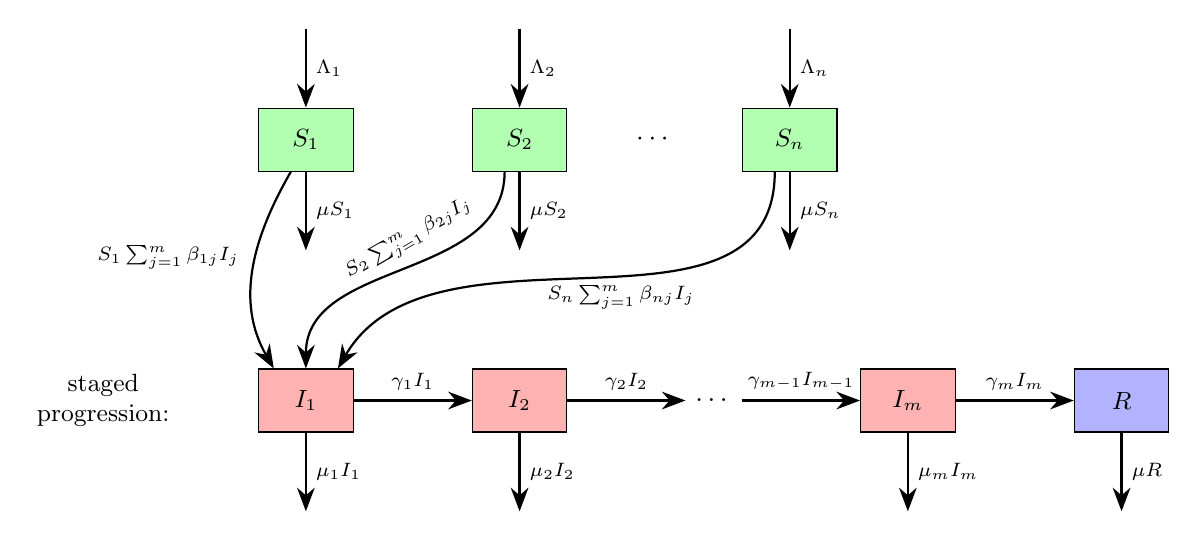
\begin{tikzpicture}[
 node distance=1.5cm,
 susceptible/.style={rectangle, draw=black, fill=green!30, minimum width=1.2cm, minimum height=0.8cm, font=\small},
 infected/.style={rectangle, draw=black, fill=red!30, minimum width=1.2cm, minimum height=0.8cm, font=\small},
 recovered/.style={rectangle, draw=black, fill=blue!30, minimum width=1.2cm, minimum height=0.8cm, font=\small},
 arrow/.style={-{Stealth[length=3mm]}, thick},
 rate/.style={font=\scriptsize}
]

% Susceptible compartments
\node[susceptible] (S1) {$S_1$};
\node[susceptible, right=of S1] (S2) {$S_2$};
\node[right=0.75cm of S2] (Sdots) {$\cdots$};
\node[susceptible, right=0.75cm of Sdots] (Sn) {$S_n$};

% Birth rates
\foreach \i in {1,2,n} {
 \draw[arrow] ([yshift=1cm]S\i.north) -- (S\i.north) node[midway, right, rate] {$\Lambda_\i$};
}

% Death rates from susceptible
\foreach \i in {1,2,n} {
 \draw[arrow] (S\i.south) -- ([yshift=-1cm]S\i.south) node[midway,
 right, rate] {$\mu {S_\i}$};
}

% Infected compartments (staged progression)
\node[infected, below=2.5cm of S1] (I1) {$I_1$};
\node[infected, right=of I1] (I2) {$I_2$};
\node[right=of I2] (Idots) {$\dots$};
\node[infected, right=of Idots] (Im) {$I_m$};

% Infection rates (from all S_i to I_1)
\draw[arrow] (S1.-115) to[out=-120, in=120] (I1.135) node[midway,
 yshift=-1.5cm, xshift=-1.75cm, rate]
% {$\beta_{11}I_1 + \beta_{12}I_2 + \cdots + \beta_{1m}I_m$};
 {$S_1\sum_{j=1}^m \beta_{1j}I_j$};
\draw[arrow] (S2.-115) to[out=-90, in=90] (I1.north) node[midway,
rotate=30, yshift=-1.75cm, xshift=0.5cm, rate]
%{$\beta_{21}I_1 + \beta_{22}I_2 + \cdots + \beta_{2m}I_m$};
 {$S_2\sum_{j=1}^m \beta_{2j}I_j$};
\draw[arrow] (Sn.-115) to[out=-90, in=60] (I1.45) node[midway,
yshift=-2.cm, xshift=4cm, rate]
%{$\beta_{n1}I_1 + \beta_{n2}I_2 + \cdots + \beta_{nm}I_m$};
 {$S_n\sum_{j=1}^m \beta_{nj}I_j$};

% Progression rates between infected classes
\draw[arrow] (I1.east) -- (I2.west) node[midway, above, rate] {$\gamma_1 I_1$};
\draw[arrow] (I2.east) -- (Idots.west) node[midway, above, rate]
{$\gamma_{2} I_{2}$};
\draw[arrow] (Idots.east) -- (Im.west) node[midway, above, rate]
{$\gamma_{m-1} I_{m-1}$};

% Death rates from infected classes
\draw[arrow] (I1.south) -- ([yshift=-1cm]I1.south) node[midway, right, rate]
{$\mu_1 {I_1}$};
\draw[arrow] (I2.south) -- ([yshift=-1cm]I2.south) node[midway, right, rate]
{$\mu_2 {I_2}$};
\draw[arrow] (Im.south) -- ([yshift=-1cm]Im.south) node[midway, right, rate]
{$\mu_m I_m$};

% Recovery compartment
\node[recovered, right=of Im] (R) {$R$};

% Recovery rate
\draw[arrow] (Im.east) -- (R.west) node[midway, above, rate] {$\gamma_m I_m$};

% Death rate from recovery
\draw[arrow] (R.south) -- ([yshift=-1.0cm]R.south) node[midway, right,
rate] {$\mu R$};

% Labels
%\node[above=2cm of S2, font=\small] {Birth rates: $\Lambda_1, \Lambda_2, \Lambda_3, \ldots, \Lambda_n$};
\node[left=1cm of I1, font=\small, align=center] {staged\\progression:};
%\node[right=2.5cm of I2, font=\small, align=center] {Death rates:\\$\mu_{I_1}, \mu_{I_2}, \ldots, \mu_{I_m}$};
\end{tikzpicture}
}
\end{figure}

\beT [\cite{IggidrCEP,Bonzi}]\lab{t:GASee} Assume that $\f( \y)=\La+ A_S \y,$ with {$A_S=-\diag[\mu_S]>0$, $\al=e_1$, and that the progression matrix $A$ has the bidiagonal progression structure in \eqref{eq: bidiagonal_A}}. If $R_0> 1$, then the unique endemic equilibrium $(\bar{S}=\fr{\La}{k \mR +\mu_S}, \bar{I})$ is globally asymptotically stable on $\Rplus^{n+m} \setminus \{(S,I) : I = 0\}$, and the function
\be{Vee} V_{EE}(\x,\y)=
 (\bff 1^t \y- \ye^t \circ \ln \y) + b (\x -\xe \circ\ln \x ), \qu b=\ye^t
\bbe (-A^{-1}):=\ye^t C
\ee
is a (Volterra type) Lyapunov function,
which has a unique global minimum at the EE $(\xe , \ye)$.
\eeT

\begin{proof} Using
\bea && \ye^t C\ba=1, C A=-\bbe\\&& \Lambda = -A_S \bar{S} + \diag(\bar{S})B \bar{I} \Lra \f(\y)=A_S(\y-\ye)+ \diag(\bar{S})B \bar{I},\eea
note that the derivative of $V_{EE}$ along trajectories of system is
\bea
V_{EE}' && =(\bff 1-\fr {\ye}{\y}).\pp{\f( \y)- \diag(\y) (\bbe \x) }+
\ye^t C \diag \pp{\bff 1-\fr {\xe}{\x}} (\ba \y^t \bbe \x+ A \x)
\\
&&=(\bff 1-\fr {\ye}{\y}).\f( \y)-\blue{\y^t (\bbe \x)}+\green{\ye^t \bbe \x}
+\blue{\y^t (\bbe \x)}- \green{\ye^t \bbe \x}
\\&& \qquad - \ye^t C \diag \pp{\fr {\xe}{\x}} (\ba \y^t \bbe \x+ A \x)
\\&&=(\bff 1-\fr {\ye}{\y}). \pp{A_S(\y-\ye)+ \diag(\bar{S})B \bar{I}}- \ye^t C \diag \pp{\fr {\xe}{\x}} \pp{\ba \y^t \bbe \x+ A \x}
\\&&=(\bff 1-\fr {\ye}{\y}). A_S(\y-\ye)+ \Omega_1+\Omega_2+\Omega_3+\Omega_4,
\eea
where
\begin{align}
\Omega_1 &=\bar{S}^t B \bar{I} = \sum_{i=1}^n \sum_{j=1}^m \beta_{ij} \bar{S}_i \bar{I}_j,\\
\Omega_2 &=-(\fr {\ye^2}{\y})^t B \bar{I} = -\sum_{i=1}^n \sum_{j=1}^m \frac{\bar{S}_i^2}{S_i}\beta_{ij} \bar{I}_j \\
\Omega_3 &=-(\y^t \bbe \x )
\ye^t B(-A)^{-1} \diag \pp{\fr {\xe}{\x}}\ba \\ \nonumber
& = -\langle B I, S \rangle (\ye^t B(-A)^{-1} \ba) \frac{\bar{I}_1}{I_1}=-\frac{\bar{I}_1}{I_1} \sum_{i=1}^n \sum_{j=1}^m \beta_{ij} I_j S_i \\ \nonumber
&= -\sum_{i=1}^n \beta_{i1} \bar{S}_i \bar{I}_1 \frac{S_i}{\bar{S}_i} - \frac{\bar{I}_1}{I_1}\sum_{i=1}^n \sum_{j=2}^m \beta_{ij} \bar{S}_i \bar{I}_j \frac{S_i}{\bar{S}_i} \frac{I_j}{\bar{I}_j} \\
\Omega_4 &=- \ye^t B(-A)^{-1} \diag \pp{\fr {\xe}{\x}} A \x.
\end{align}

Each $\Omega_i$ represents a distinct biological and mathematical aspect:

\begin{itemize}
\item $\Omega_1$: Direct transmission effect at equilibrium
\item $\Omega_2$: Correction for deviation of susceptible populations from equilibrium
\item $\Omega_3$: Effect of new infections entering the first infected stage
\item $\Omega_4$: Staged progression effects through the infected compartments
\end{itemize}

Finally, Bonzi shows that the sum of the four omegas may be written as:
\be{Bid} \bc
\sum_{i=1}^4 \Omega_i &= \sum_{i=1}^n \beta_{i1} \bar{S}_i \bar{I}_1 \left(2 - \frac{\bar{S}_i}{S_i} - \frac{S_i}{\bar{S}_i}\right) \\
&\quad + \sum_{i=1}^n \sum_{j=2}^m \beta_{ij} \bar{S}_i \bar{I}_j \left[j + 1 - \frac{\bar{S}_i}{S_i} - \frac{S_i}{\bar{S}_i} \frac{\bar{I}_1}{I_1} \frac{I_j}{\bar{I}_j} - \sum_{k=1}^{j-1} \frac{I_k}{\bar{I}_k} \frac{\bar{I}_{k+1}}{I_{k+1}}\right]\ec
\ee
and that it is always non-positive, and strictly negative if $(\x,\y) \neq (\xe,\ye)$. Global asymptotic stability thus follows. The last step is quite intricate, and we have provided a check in the Mathematica file BonziEE.nb.
\end{proof}

\fi


\end{document}

